\documentclass[11pt,a4paper]{article}
\usepackage[utf8]{inputenc}
\usepackage[T1]{fontenc}
\usepackage{amsthm} %numéroter les questions
% \usepackage[frenchb]{babel}
\usepackage{datetime}
\usepackage{xspace} % typographie IN
\usepackage{hyperref}% hyperliens
\usepackage[all]{hypcap} %lien pointe en haut des figures
\usepackage[french]{varioref} %voir x p y
\usepackage{fancyhdr}% en têtes
%\input cyracc.def
\usepackage[]{graphicx} %include pictures
\usepackage{pgfplots}
\usepackage[ ]{circuitikz}
\usepackage{ifthen}

\usepackage[top=1.3 in, bottom=1.3 in, left=1.3 in, right=1.3 in]{geometry} % Yeah, that's bad to play with margins
\usepackage[]{pdfpages}

\usepackage[]{attachfile}

\usepackage{float}

\newdateformat{mydate}{v2.0.1}%hack pour remplacer \THEYEAR


\newboolean{corrige}
\ifx\correction\undefined
\setboolean{corrige}{false}% pas de corrigé
\else
\setboolean{corrige}{true}%corrigé
\fi

\setboolean{corrige}{false}% pas de corrigé

\newboolean{annexes}
\setboolean{annexes}{true}%annexes
%\setboolean{annexes}{false}% pas de annexes

\definecolor{darkblue}{rgb}{0,0,0.5}

\newboolean{mos}
%\setboolean{mos}{true}%annexes
\setboolean{mos}{false}% pas de annexes

\usepackage{aeguill} %guillemets

%% fancy header & foot
\pagestyle{fancy}
%Numero du TP:
\def \labonumber {Laboratory work 2 }
\lhead{[ELEC-H-310] Digital Choucroute\\ \labonumber}
\rhead{\mydate\today\\ page \thepage}
\chead{\ifthenelse{\boolean{corrige}}{Corrigé}{}}
\cfoot{}
%%

\pdfinfo{
/Author (ULB -- BEAMS)
/Title (\labonumber ELEC-H-310)
/ModDate (D:\pdfdate)
}

\hypersetup{
pdftitle={\labonumber [ELEC-H-310] Digital Choucroute},
pdfauthor={ULB -- BEAMS},
pdfsubject={}
}

\theoremstyle{definition}% questions pas en italique
\newtheorem{Q}{Question}[] % numéroter les questions [section] ou non []

\newcommand{\reponse}[1]{% pour intégrer une réponse: \reponse{texte}: sera inclus si \boolean{corrige}
	\ifthenelse {\boolean{corrige}} {\paragraph{Answer:} \color{darkblue}   #1\color{black}} {}
 }

\newcommand{\addcontentslinenono}[4]{\addtocontents{#1}{\protect\contentsline{#2}{#3}{#4}{}}}

\date{\vspace{-1.7cm}\mydate\today}
\title{\vspace{-2cm} \labonumber\\ Digital Electronics [ELEC-H-310]\\Realization of a synthetizer\ifthenelse{\boolean{corrige}}{\\Solution}{}}

%\author{\vspace{-1cm}}%\textsc{Yannick Allard}}

\setlength{\parskip}{0.2cm plus2mm minus1mm} %espacement entre §
\setlength{\parindent}{0pt}

\begin{document}
\pagestyle{empty}
\maketitle
% \vspace*{-1cm}
\section*{Purpose}
The main purpose of this manipulation is to create a complex digital system: a sound synthetizer.
To implement it, you must understand the functioning of the analog-to-digital converter (ADC) as well as the digital-to-analog converter (DAC).

\section*{Prerequisite}
Before the lab, we advise you to read sections\ref{sec:intro} and \ref{sec:predet} of this lab. Also watch the tutorial on interrupts on \url{https://www.cypress.com/video-library/PSoC-Software/psoc-101-lesson-3-interrupts/387711}. 

Also make sure to \textbf{bring} some 3.5mm jack \textbf{headphones} in order to listen to what you will be programming.

\section*{Predeterminations}
You are asked to answer exercices of section\ref{sec:predet}.

\section*{Objectives}
At the end of this lab, you must be able to:
\begin{itemize}
	\item Write a program for a microcontroller.
	\item Explain the functioning of an analog-to-digital converter.
	\item Explain the usefulness of the interrupt.
	\item Link the specifications to the peripherals of a microcontoller.
\end{itemize}

\newpage{}

\section{Introduction to the analog-to-digital conversion}
\label{sec:intro}

\subsection{Introduction}
Microprocessors are present in practically every industrial processes (temperature control, speed display, alarm systems) as well as in our common life (alarm-radio, audio systems, etc.).
All those processes have in common the interaction with analog variables (see figure\ref{fig:arch-processus}).
Processors work with digital variables thus, it is necessary to convert those physical analog quantities into digital values and inversely.

The transformation of physical signal to digital is done in two steps:
\begin{enumerate}
	\item Conversion of the physical signal to measure (temperature, speed, ...) into voltage. It is the role of the sensor (thermocouple, accelerometer, etc.).
	\item Conversion of this voltage into binary value. It is the role of the analog-to-digital converter (ADC).
\end{enumerate}

The reversed path allows to convert a digital number to a physical quantity:
\begin{enumerate}
	\item The digital-to-analog converter (DAC) transforms a binary number into voltage.
	\item The actuator converts the voltage into another physical quantity that will activate some system (\textit{e.g.} microwaves, electrical drives, gates, motors, etc.).
\end{enumerate}

\begin{figure}[H]
	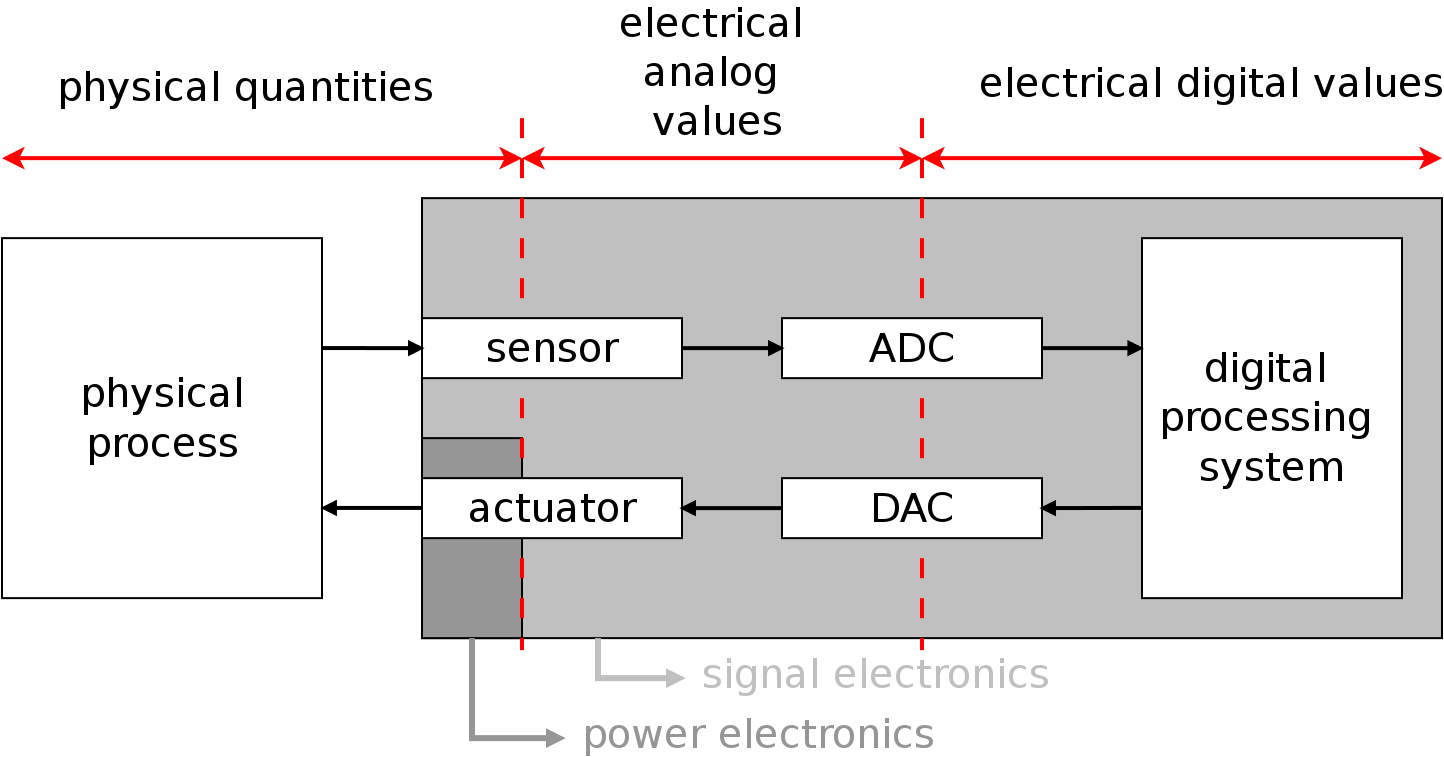
\includegraphics[width=\textwidth]{ENarch-processus}
	\caption{Architecture of a process}
	\label{fig:arch-processus}
\end{figure}

\subsection{Analog-to-digital conversion}
The analog-to-digital converter turns an analog voltage (changing continuously) into a digital number coded on a fixed value of bits (8 to 20 bits for the PSOC).
To do so, the converter does a double quantization (see figure\ref{fig:double-quant}):
\begin{itemize}
	\item Time quantization, also called sampling.
	\item Level quantization.
\end{itemize}
Note that it is impossible to perfectly represent an analog signal into a finite number of bits.

\begin{figure}[H]
	\centering
	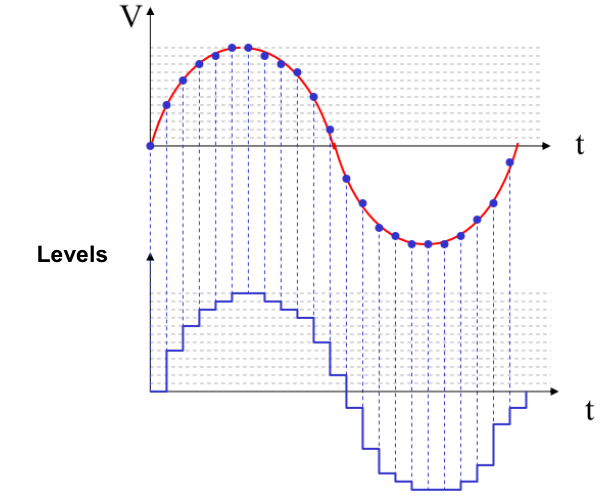
\includegraphics[width=.7\textwidth]{ENdouble-quant}
	\caption{Double quantization}
	\label{fig:double-quant}
\end{figure}

The performances of an ADC depend mostly on two parameters:
\begin{itemize}
	\item The sampling frequency.
	\item The resolution, in other words the number N of bits coding the converted value.
    The resolution can be electrically defined as the smallest detectable change of voltage.
    If the converter has an operating range from 0V to 5V and convert the quantity on 10 bits, the resolution is $\frac{5 V}{2^{10}-1} = 4,9 mV$(\textit{i.e.} input range).
    Finally, each binary number coded on N bits will correspond to an input voltage range.

\end{itemize}

\begin{figure}
	\centering
	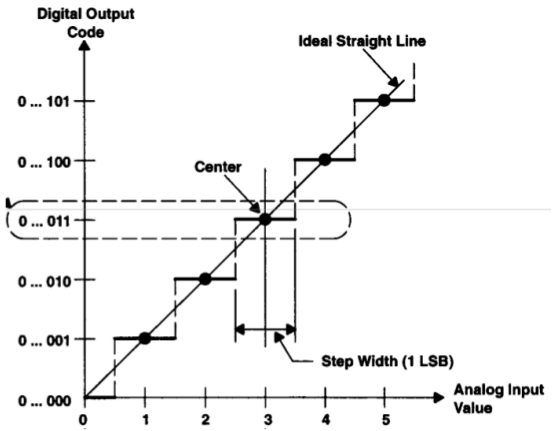
\includegraphics[width=.7\textwidth]{an-dig}
	\caption{Digital coding of an analog value}
	\label{fig:an-dig}
\end{figure}

\subsection{Digital-to-analog conversion}
Its principle is the opposite of the ADC: the transformation of a number coded on N bits to a voltage in its output range.
The voltage obtained is continuous in time (the output of the converter is constant until a new conversion is done), but is always quantized because only $2^N$ different voltage values are achievable (each binary code correspond to one voltage).



\section{Predeterminations}\label{sec:predet}
\begin{enumerate}
	\item Compute the resolution of ADC present on the PSOC board knowing that the input voltage range is 0-5V and that we will use the ADC with 16 bits.
	\item Determine the memory space needed to store an audio file of 3s, sampled at 11kHz, knowing one sample is stored on one byte.
\end{enumerate}



\section{Manipulation}

\subsection{Realization of a voltmeter}
First of all, you will familiarize yourselves with the use of the ADC with a simple application: a voltmeter measuring the voltage on a potentiometer connected to input \texttt{P0[7]} (see file ``Extension PSOC'').
A feedback will be done using the LEDs as a bar graph (the higher the voltage, the more LEDs are switched on)
The ADC must sample at rate of 10kHz.
\begin{itemize}
	\item Draw the block diagram of the whole system.
	Which peripheral will be used?
    Highlight the interfaces between the inside and outside of the $\mu$C by separating them clearly.
	\item Instantiate an (analog) input pin for the signal coming from the potentiometer in the topDesign.cysch file.
	\item Instantiate a Delta-Sigma ADC in the topDesign.cysch file. The ADC should sample at 10kHz with a resolution of 16 bits. Since the signal we are measuring has the same ground as the PSOC board, the ADC should be set to Single-ended mode rather than differential.
	This setting can be found in the ``Common" tab, in the ``Input mode" frame.
	\item Using the ADC datasheet Application Programming Interface section, determine which function you should call from the firmware (i.e. the main.c file) to determine whether the ADC has finished it's current conversion. 
	\item Using the ADC datasheet Application Programming Interface section, determine which function you should call from the firmware (i.e. the main.c file) to read the ADC value. Should you use the 16- or 32-bit version of the function? 
	\item Now write the firmware code (i.e. the main.c file code) to check whether the ADC is finished converting, read the ADC value, and light the appropriate number of LEDs depending on which value was read (for reminder: a high ADC value should light all LEDs, while a low ADC value should light no LEDs). Don't forget to start your ADC before the infinite loop! 
\end{itemize}





\subsection{Synthesizer}
A synthesizer is a device capable of generating an arbitrary sound wave and convert it to sound through a speaker.
In our case, we will simply generate a sine wave at adjustable frequency: the processor will send samples corresponding to the wanted waveform to a DAC and once rebuilt, the signal will be sent to the amplifier of the extension board.
\begin{itemize}
	\item During the configuration of your peripherals (before the infinite loop), fill the wave vector (of length 100) defined as global variable so that it contains one full period of a sine wave defined between -1 and +1.
    To do so, you must:
	\begin{itemize}
		\item include the file math.h in the header (you also need to add it in the linker settings, see Figure~\ref{fig:linker});
		\item call function sin(), that takes as argument a floating number representing the angle (in rad) and that also returns a floating number.
	\end{itemize}
	\item Program a timer so that a sample of the sine wave is processed every 50$\mu$s
	\item Instantiate an (analog) output pin of the DAC in the topDesign.cysch file, and connect it to the DAC\_OUT pin of the extension board (see ``Extension PSOC'' file). 
	\item Instantiate a VDAC in the topDesign.cysch file. The range is from 0 to 1.020V and a slow speed is sufficient. Make sure you select ``CPU'' as the data source, since we will provide the data from the firmware (i.e. the main.c file). The strobe should be set to ``Register Write'', which means the DAC will provide a new analog value every time a new value is written in it's register. 
	\item In your firmware code (i.e. the main.c file), poll the timer to detect timer overflows (as done in the previous lab). Every 50$\mu$s, write the next value of the sine wave vector to the DAC by using the appropriate command (that you can find in the VDAC datasheet Application Programming Interface). Note that the DAC expect to see an 8-bit signal (i.e. between 0 and 255), so you should shift (center around 128) and scale (amplitude between 0 and 128) your sine wave so that it remains within this range at all times. Don't forget to start your DAC before the infinite loop! 
	\item Add a volume control by coupling the measure from the potentiometer (representing the volume) with your synthesizer.
\end{itemize}

\begin{figure}
\centering
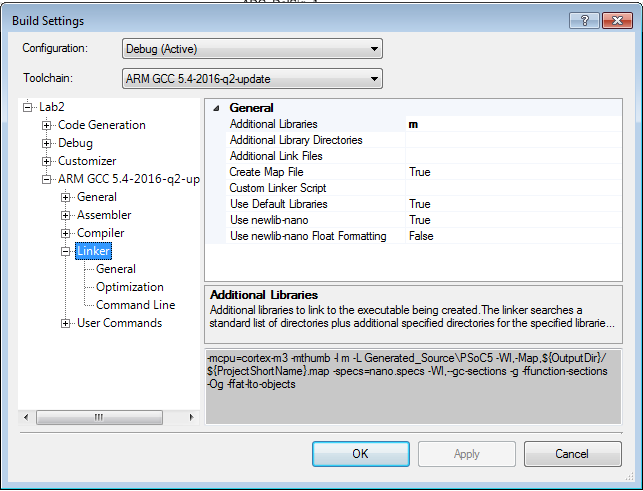
\includegraphics[width=12cm]{linker-settings.png}
\caption{To compile with the \texttt{math.h} library, add ``m" in the ``Additional Libraries" field. This windows is found under \texttt{Project > Build Settings...}.}
\label{fig:linker}
\end{figure}




\subsection{Interrupts}

We will now study how we can use interrupts in our code to generate super-priority events. When an interrupt is latched, the firmware is temporarily interrupted while the Interrupt Service Routine (ISR) is executed. Watch the tutorial on \url{https://www.cypress.com/video-library/PSoC-Software/psoc-101-lesson-3-interrupts/387711} to see how to program interrupts with PSOC. 
\begin{itemize}
	\item Take your previous project. 
	\item To write the data to the DAC from the firmware, we will now create an Interrupt. Instantiate an Interrupt in the topDesign.cysch file, and connect it to the interrupt-output of the timer. This means that every time the timer overflows, this interrupt will be triggered. 
	\item Following the video tutorial on interrupts, write your firmware so that your code that was previously inside your polling-loop is now in your ISR (don't forget to remove/comment out the polling of the timer). Read the documentation about the interrupt output in the timer datasheet. Is there something special you should do at the end of your ISR? 
	\item Similarly to the previous exercise, add a volume control by coupling the measure from the potentiometer (representing the volume) with your synthesizer.
\end{itemize}
	

\end{document}
